\chapter{Ácidos y bases: Ka y pKa}\label{ch:g12:ka-and-pka}

Muchas hormigas se defienden con ácido metanoico, que quema la piel. El
ácido metanoico es un \omterm{def:g11:functional-groups:carboxylic-acid}{ácido
carboxílico} pequeño. El ácido clorhídrico a la misma concentración
quemaría mucho más. Los dos son ácidos; los dos dan una disolución de \omterm{def:g9:acids-bases-ph:ph}{pH}
inferior a 7; y, sin embargo, no son ácidos de la misma manera. Para
describir un ácido por completo hacen falta dos números: cuánto hay, su
concentración, y con qué facilidad cede su \omterm{def:g9:ions:ion}{ion} hidrógeno, su \omterm{def:g12:ka-and-pka:ka}{constante de
acidez}.

\begin{recall}
Las \omterm{def:g9:acids-bases-ph:acidic}{disoluciones ácidas}, básicas y neutras; la escala de \omterm{def:g9:acids-bases-ph:ph}{pH}, de 0 a 14,
más baja cuantos más \omterm{def:g9:ions:ion}{iones} hidrógeno hay (\cref{ch:g9:acids-bases-ph}). El
\omterm{def:g12:equilibrium:quotient}{cociente de reacción} $Q$ y la \omterm{def:g12:equilibrium:constant}{constante de equilibrio} $K$
(\cref{ch:g12:equilibrium}). Una \omterm{def:g12:curly-arrows:curly-arrow}{flecha curva} representa el
desplazamiento de un par de \omterm{def:g9:inside-the-atom:nucleus}{electrones} (\cref{ch:g12:curly-arrows}).
\end{recall}

\begin{omfigure}
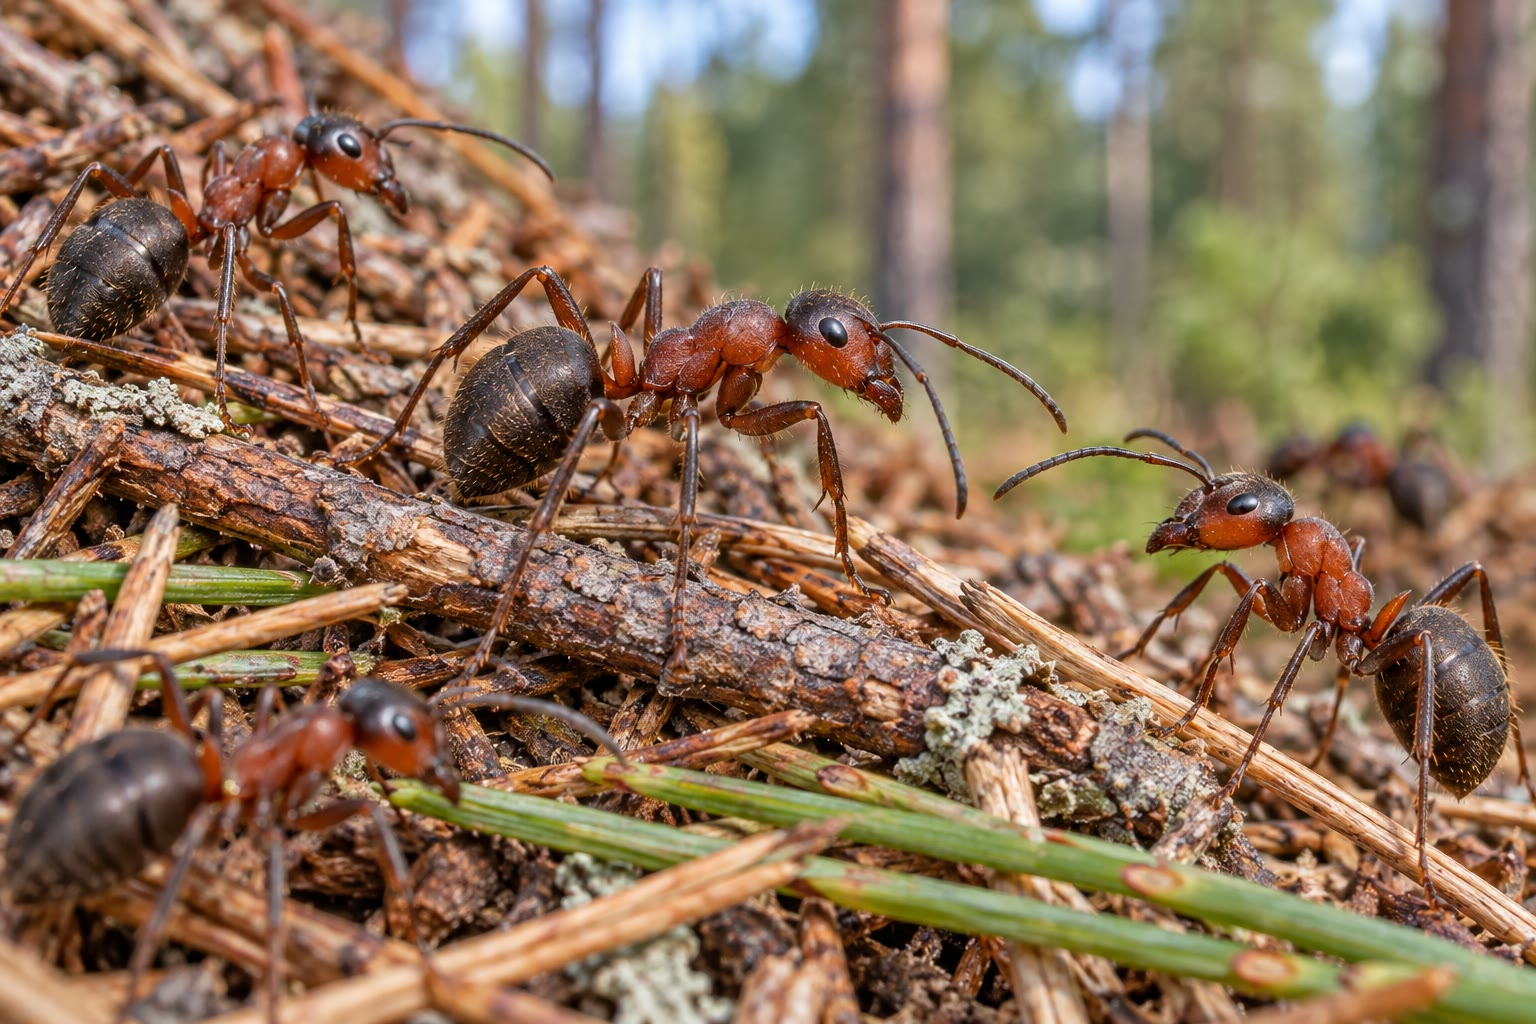
\includegraphics[width=0.45\linewidth]{images/book1/ai/g12-red-ants.jpg}

{\small Hormigas de los bosques: como muchas hormigas, se defienden con
ácido metanoico.}
\end{omfigure}

\section{Ácidos y bases de Brønsted}

\begin{definition}[Ácido y base de Brønsted, par ácido--base]\label{def:g12:ka-and-pka:bronsted}
Un \emph{ácido de Brønsted}\index{acido de Bronsted@ácido de Brønsted} es una especie capaz
de ceder un \omterm{def:g9:ions:ion}{ion} hidrógeno \ce{H+}; una \emph{base de Brønsted}\index{base de Bronsted@base de Brønsted}
es una especie capaz de captarlo. Un ácido HA y la base \ce{A-} en la que
se convierte al perder \ce{H+} forman un \emph{par ácido--base}\index{par acido--base@par ácido--base},
que se escribe \ce{HA}/\ce{A-}: $\ce{HA} \rightleftharpoons \ce{A-} + \ce{H+}$.
\end{definition}

\begin{definition}[Ion oxonio, anfolito]\label{def:g12:ka-and-pka:oxonium}
En el agua, un \omterm{def:g9:ions:ion}{ion} hidrógeno nunca queda solo: lo capta una \omterm{def:g7:atoms-and-molecules:molecule}{molécula} de
agua, lo que da el \emph{ion oxonio}\index{ion oxonio} \ce{H3O+}. Una
especie que es el ácido de un par y la base de otro es un
\emph{anfolito}\index{anfolito}; el agua lo es: ácido del par
\ce{H2O}/\ce{OH-} y base del par \ce{H3O+}/\ce{H2O}.
\end{definition}

\begin{example}[Un ácido en el agua]\label{ex:g12:ka-and-pka:acid-water}
Cuando el ácido etanoico se \omterm{def:g2:mixing-and-dissolving:dissolve}{disuelve}, un \omterm{def:g10:lewis-and-shape:lone-pair}{par libre} de una \omterm{def:g7:atoms-and-molecules:molecule}{molécula} de
agua capta el hidrógeno de su \ce{O-H}, y el par \ce{O-H} se queda en el
oxígeno del ácido:
\[
  \ce{CH3COOH + H2O <=> CH3COO- + H3O+} .
\]
Dos pares intercambian un \omterm{def:g9:ions:ion}{ion} hidrógeno: \ce{CH3COOH}/\ce{CH3COO-} lo
cede y \ce{H3O+}/\ce{H2O} lo capta. A partir de ahora, los \omterm{def:g9:ions:ion}{iones}
hidrógeno de los capítulos anteriores se escriben \ce{H3O+} siempre que el
agua sea el \omterm{def:g6:solutions-and-solubility:solute}{disolvente}.
\end{example}

\begin{omfigure}
\setchemfig{atom sep=2em}
\chemfig{H_3C-C(=[2]O)-O-[@{oh}]@{h}H}\qquad
\chemfig{@{ow}\charge{90=\:,270=\:}{O}(-[:150]H)-[:210]H}
\qquad$\longrightarrow$\qquad
\chemfig{H_3C-C(=[2]O)-\charge{90=\:,0=\:,270=\:}{O}^{-}}\quad$+$\quad\ce{H3O+}
\chemmove{
  \draw[->, thick, omProp, shorten <=4pt, shorten >=3pt]
    ($(ow)+(0,0.25)$) .. controls +(110:9mm) and +(60:9mm) .. (h);
  \draw[->, thick, omDef, shorten <=2pt, shorten >=4pt]
    (oh) .. controls +(-90:7mm) and +(-60:6mm) .. ($(oh)+(-0.3,-0.2)$);}

{\small Un \omterm{def:g9:ions:ion}{ion} hidrógeno pasa del ácido al agua: un \omterm{def:g10:lewis-and-shape:lone-pair}{par libre} del agua
forma el nuevo enlace \ce{O-H} (en naranja), y el antiguo par \ce{O-H} se
queda en el oxígeno del \omterm{def:g9:ions:ion}{ion} etanoato (en azul).}
\end{omfigure}

\begin{history}[De Arrhenius a Brønsted, 1887--1923]
En 1887, Svante Arrhenius propuso que los ácidos liberan \omterm{def:g9:ions:ion}{iones} hidrógeno
en el agua, y las bases, \omterm{def:g9:ions:ion}{iones} hidróxido. En 1923, Johannes Brønsted y,
de forma independiente, Thomas Lowry ampliaron la idea: un ácido es
cualquier especie que cede un \omterm{def:g9:ions:ion}{ion} hidrógeno, y una base, cualquier
especie que lo capta, en el agua o fuera de ella. La \omterm{def:g7:atoms-and-molecules:molecule}{molécula} de
amoníaco, que no contiene hidróxido, pasó a ser una base como las demás.
\end{history}

\begin{omfigure}
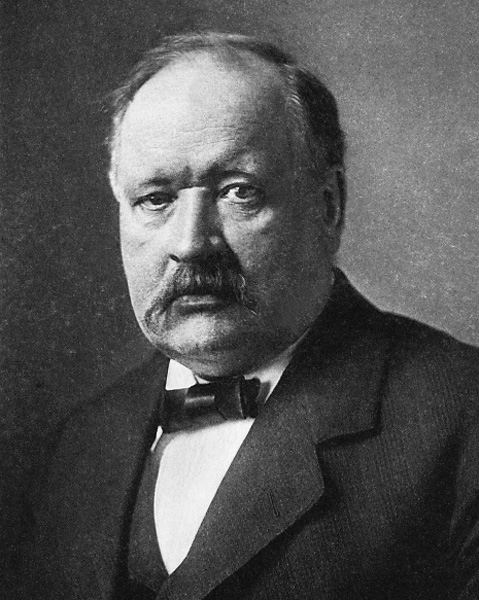
\includegraphics[width=0.22\linewidth]{images/book1/arrhenius.jpg}

{\small Svante Arrhenius (1859--1927).}
\end{omfigure}

\section{El pH, cuantitativamente}

\begin{definition}[El pH, con precisión]\label{def:g12:ka-and-pka:ph-log}
En una \omterm{def:g6:solutions-and-solubility:solute}{disolución acuosa} diluida, el \omterm{def:g9:acids-bases-ph:ph}{pH} se define por
\[
  \mathrm{pH} = -\log\frac{[\ce{H3O+}]}{c^\circ},
  \qquad\text{es decir}\qquad
  [\ce{H3O+}] = c^\circ \times 10^{-\mathrm{pH}} ,
\]
donde $\log$ es el logaritmo decimal.
\end{definition}

\begin{proposition}[Dilución por diez, una unidad]\label{prop:g12:ka-and-pka:dilution}
Si $[\ce{H3O+}]$ se divide por 10, el \omterm{def:g9:acids-bases-ph:ph}{pH} aumenta en 1; si se multiplica
por 10, el \omterm{def:g9:acids-bases-ph:ph}{pH} disminuye en 1.
\end{proposition}

\begin{proof}
$-\log\big([\ce{H3O+}]/10c^\circ\big) = -\log\big([\ce{H3O+}]/c^\circ\big)
+ \log 10 = \mathrm{pH} + 1$.
\end{proof}

\begin{definition}[Ácidos y bases fuertes y débiles]\label{def:g12:ka-and-pka:strong-acid}
Un \emph{ácido fuerte}\index{acido fuerte@ácido fuerte} reacciona totalmente con el
agua: no queda nada del ácido como tal en la disolución. Un \emph{ácido
débil}\index{acido debil@ácido débil} reacciona parcialmente: su reacción con el agua
alcanza un equilibrio. Del mismo modo, una \emph{base fuerte}\index{base fuerte}
reacciona totalmente con el agua, y una \emph{base débil}\index{base debil@base débil},
parcialmente.
\end{definition}

\begin{proposition}[pH de un ácido fuerte]\label{prop:g12:ka-and-pka:strong}
Una disolución de un \omterm{def:g12:ka-and-pka:strong-acid}{ácido fuerte} de concentración $c$ (no demasiado
diluida) tiene $[\ce{H3O+}] = c$ y $\mathrm{pH} = -\log(c/c^\circ)$.
\end{proposition}

\begin{proof}
La reacción \ce{HA + H2O -> A- + H3O+} es total: cada \omterm{def:g7:atoms-and-molecules:molecule}{molécula} de ácido
da un \omterm{def:g12:ka-and-pka:oxonium}{ion oxonio}. Los \omterm{def:g9:ions:ion}{iones} procedentes del propio agua son despreciables
mientras $c$ sea mucho mayor que \qty{e-7}{mol/L}.
\end{proof}

\begin{example}[El ácido clorhídrico]\label{ex:g12:ka-and-pka:hcl}
Ácido clorhídrico a \qty{0.010}{mol/L}: $[\ce{H3O+}] = \qty{0.010}{mol/L}$
y $\mathrm{pH} = -\log 0.010 = 2.0$. Diluido diez veces, \omterm{def:g9:acids-bases-ph:ph}{pH} 3.0.
\end{example}

\section{El agua y el producto iónico}


\begin{definition}[Producto iónico del agua]\label{def:g12:ka-and-pka:ionic-product}
El agua reacciona muy ligeramente consigo misma, \ce{2H2O <=> H3O+ + OH-}.
La \omterm{def:g12:equilibrium:constant}{constante de equilibrio} de esta reacción es el \emph{producto iónico
del agua}\index{producto ionico del agua@producto iónico del agua}:
\[
  K_e = \frac{[\ce{H3O+}]\,[\ce{OH-}]}{(c^\circ)^2},
  \qquad pK_e = -\log K_e .
\]
\end{definition}

\begin{proposition}[El agua neutra y las bases fuertes]\label{prop:g12:ka-and-pka:ke}
% ledger: ke:25C
A \qty{25}{\celsius}, $K_e = \num{1.0e-14}$ y $pK_e = 14.0$. En el agua
pura, $[\ce{H3O+}] = [\ce{OH-}] = \qty{1.0e-7}{mol/L}$: \omterm{def:g9:acids-bases-ph:ph}{pH} 7.0. Una \omterm{def:g12:ka-and-pka:strong-acid}{base
fuerte} de concentración $c$ da $[\ce{OH-}] = c$, así que
$[\ce{H3O+}] = K_e (c^\circ)^2 / c$ y $\mathrm{pH} = 14.0 + \log(c/c^\circ)$.
\end{proposition}

\begin{proof}
En el agua pura, los dos \omterm{def:g9:ions:ion}{iones} se forman a pares, así que son iguales, y
su producto es $\num{1.0e-14}$: cada uno vale \qty{1.0e-7}{mol/L}. Para
la base, $K_e$ sigue cumpliéndose en la disolución:
$-\log([\ce{H3O+}]/c^\circ) = -\log K_e + \log(c/c^\circ)$.
\end{proof}

\begin{example}[El hidróxido de sodio]\label{ex:g12:ka-and-pka:naoh}
Hidróxido de sodio a \qty{0.010}{mol/L}: $[\ce{OH-}] = 0.010$, así que
$[\ce{H3O+}] = \num{1.0e-14}/0.010 = \qty{1.0e-12}{mol/L}$ y \omterm{def:g9:acids-bases-ph:ph}{pH} 12.0.
\end{example}

\section{La constante de acidez}

\begin{definition}[Constante de acidez, $pK_a$]\label{def:g12:ka-and-pka:ka}
La \emph{constante de acidez}\index{constante de acidez} $K_a$ de un par
\ce{HA}/\ce{A-} es la \omterm{def:g12:equilibrium:constant}{constante de equilibrio} de la reacción del ácido
con el agua, \ce{HA + H2O <=> A- + H3O+}:
\[
  K_a = \frac{[\ce{A-}]\,[\ce{H3O+}]}{[\ce{HA}]\,c^\circ} .
\]
El \emph{pKa}\index{pKa} del par es
$pK_a = -\log K_a$.
\end{definition}

\begin{proposition}[Cuanto menor es el $pK_a$, más fuerte es el ácido]\label{prop:g12:ka-and-pka:compare}
De dos \omterm{def:g12:ka-and-pka:strong-acid}{ácidos débiles} a la misma concentración, el de mayor $K_a$, es
decir, el de menor $pK_a$, reacciona más con el agua y da el \omterm{def:g9:acids-bases-ph:ph}{pH} más
bajo; su base conjugada es la más débil.
\end{proposition}

\begin{proof}
Una $K_a$ mayor significa más \ce{A-} y más \ce{H3O+} en el equilibrio
para la misma cantidad de \ce{HA}. La base \ce{A-} de un par que cede
fácilmente su \omterm{def:g9:ions:ion}{ion} hidrógeno lo recupera con dificultad.
\end{proof}

\begin{omfigure}
\begin{tikzpicture}[font=\small, y=0.55cm]
  % ledger: pka:methanoic, pka:ethanoic, pka:benzoic, pka:ascorbic1, ka:HF, ka:H2CO3, ka:HCO3, kb:NH3, ke:25C
  \draw[->, thick] (0,0) -- (0,14.8) node[above] {$pK_a$};
  \foreach \k in {0,2,4,6,8,10,12,14} \draw (-0.1,\k) -- (0.1,\k) node[right, font=\scriptsize] {\k};
  \node[font=\footnotesize\bfseries, anchor=south] at (-3.0,14.3) {ácido};
  \node[font=\footnotesize\bfseries, anchor=south] at (3.0,14.3) {base};
  \foreach \p/\yl/\acid/\base in {3.19/2.9/{\ce{HF}}/{\ce{F-}},
      3.74/3.6/{\ce{HCOOH}}/{\ce{HCOO-}}, 4.04/4.3/{ácido ascórbico}/{ascorbato},
      4.20/5.0/{\ce{C6H5COOH}}/{\ce{C6H5COO-}}, 4.76/5.7/{\ce{CH3COOH}}/{\ce{CH3COO-}},
      6.37/6.9/{\ce{CO2,H2O}}/{\ce{HCO3-}}, 9.26/9.26/{\ce{NH4+}}/{\ce{NH3}},
      10.33/10.4/{\ce{HCO3-}}/{\ce{CO3^{2-}}}} {
    \draw[omDef] (-0.25,\p) -- (0.25,\p);
    \draw[black!40] (-0.25,\p) -- (-1.1,\yl);
    \draw[black!40] (0.25,\p) -- (1.1,\yl);
    \node[anchor=east, font=\scriptsize] at (-1.15,\yl) {\acid};
    \node[anchor=west, font=\scriptsize] at (1.15,\yl) {\base};
  }
  \draw[->, omThm, thick] (-4.6,13) -- (-4.6,1);
  \node[omThm, rotate=90, font=\footnotesize] at (-4.95,7) {ácidos más fuertes};
  \draw[->, omMeth, thick] (4.6,1) -- (4.6,13);
  \node[omMeth, rotate=90, font=\footnotesize] at (4.95,7) {bases más fuertes};
\end{tikzpicture}

{\small Algunos pares situados según su $pK_a$ a \qty{25}{\celsius}, con
los ácidos a la izquierda y sus bases a la derecha. Cuanto más abajo está
un par en la escala, más fuerte es su ácido; cuanto más arriba, más
fuerte es su base.}
\end{omfigure}


\begin{method}[pH de un ácido débil]\label{met:g12:ka-and-pka:weak}
Para un \omterm{def:g12:ka-and-pka:strong-acid}{ácido débil} de concentración $c$ y constante $K_a$:
\begin{enumerate}
  \item Escribe la \omterm{def:g10:reaction-progress-table:extent}{tabla de avance} de \ce{HA + H2O <=> A- + H3O+} por
        litro, con $x = [\ce{H3O+}]$: $[\ce{HA}] = c - x$, $[\ce{A-}] = x$
        (despreciando los \omterm{def:g9:ions:ion}{iones} propios del agua).
  \item Resuelve $\dfrac{x^2}{(c - x)\,c^\circ} = K_a$, la ecuación de
        segundo grado $x^2 + K_a c^\circ x - K_a c^\circ c = 0$,
        quedándote con la raíz positiva.
  \item $\mathrm{pH} = -\log(x/c^\circ)$; comprueba que $x$ es mucho
        mayor que \qty{e-7}{mol/L}.
\end{enumerate}
\end{method}

\begin{example}[Ácido etanoico a \texorpdfstring{\qty{0.010}{mol/L}}{0.010 mol/L}]\label{ex:g12:ka-and-pka:acetic}
% ledger: pka:ethanoic
$pK_a = 4.76$, así que $K_a = 10^{-4.76} = \num{1.74e-5}$. Entonces
$x^2 + \num{1.74e-5}\,x - \num{1.74e-7} = 0$ da
$x = \qty{4.1e-4}{mol/L}$ y \omterm{def:g9:acids-bases-ph:ph}{pH} 3.39. Solo el $\num{4.1e-4}/0.010 =
\qty{4.1}{\percent}$ del ácido ha reaccionado con el agua; el ácido
clorhídrico a la misma concentración, de \omterm{def:g9:acids-bases-ph:ph}{pH} 2.0, ha reaccionado por
completo.
\end{example}

\begin{omfigure}
\begin{tikzpicture}[font=\small]
  \fill[omThm!45] (0,1.3) rectangle (8,2.0);
  \node[anchor=east] at (-0.1,1.65) {\ce{HCl}, \qty{0.010}{mol/L}};
  \node[white, font=\small\bfseries] at (4,1.65) {\ce{H3O+} + \ce{Cl-}: \qty{100}{\percent}};
  \fill[omDef!35] (0,0) rectangle (7.67,0.7);
  \fill[omThm!45] (7.67,0) rectangle (8,0.7);
  \node[anchor=east] at (-0.1,0.35) {\ce{CH3COOH}, \qty{0.010}{mol/L}};
  \node at (3.8,0.35) {\ce{CH3COOH} sin reaccionar: \qty{95.9}{\percent}};
  \draw[<-, omThm] (7.85,0.75) -- (8.4,1.1) node[right, font=\footnotesize] {\qty{4.1}{\percent} ionizado};
\end{tikzpicture}

{\small Qué ocurre con un \omterm{def:g12:ka-and-pka:strong-acid}{ácido fuerte} y con uno débil a la misma
concentración: el \omterm{def:g12:ka-and-pka:strong-acid}{ácido fuerte} se transforma por completo en \omterm{def:g9:ions:ion}{iones}; el
débil, apenas. De ahí la diferencia de \omterm{def:g9:acids-bases-ph:ph}{pH}, 2.0 frente a 3.4.}
\end{omfigure}

\begin{safety}{\ghs[0.75cm]{GHS02}\ghs[0.75cm]{GHS05}\ghs[0.75cm]{GHS06}\ghs[0.75cm]{GHS07}}
% ledger: ghs:formic-acid
El ácido metanoico concentrado es inflamable, provoca quemaduras graves
en la piel y en los ojos, y su vapor es tóxico. Solo lo manipula el
profesor, bajo una campana de \omterm{def:g10:chemical-species:extraction}{extracción}; las disoluciones diluidas de
los ejercicios también exigen gafas.
\end{safety}

\section{Ejercicios}

\begin{exercise}[$\star$]\label{exo:g12:ka-and-pka:1}
Da la base conjugada de: \ce{HCOOH}, \ce{NH4+}, \ce{H2O}, \ce{HCO3-}; y
el ácido conjugado de: \ce{NH3}, \ce{OH-}, \ce{H2O}, \ce{HCO3-}. ¿Qué
especies son \omterm{def:g12:ka-and-pka:oxonium}{anfolitos}?
\end{exercise}

\begin{exercise}[$\star$]\label{exo:g12:ka-and-pka:2}
Calcula el \omterm{def:g9:acids-bases-ph:ph}{pH} del ácido clorhídrico a \qty{0.10}{mol/L},
\qty{0.0010}{mol/L} y \qty{5.0e-3}{mol/L}.
\end{exercise}

\begin{exercise}[$\star$]\label{exo:g12:ka-and-pka:3}
Una disolución tiene \omterm{def:g9:acids-bases-ph:ph}{pH} 4.5. Calcula $[\ce{H3O+}]$. Una disolución tiene
\omterm{def:g9:acids-bases-ph:ph}{pH} 11.2: calcula $[\ce{H3O+}]$ y $[\ce{OH-}]$ a \qty{25}{\celsius}.
\end{exercise}

\begin{exercise}[$\star$]\label{exo:g12:ka-and-pka:4}
Escribe la reacción con el agua y la expresión de $K_a$ para el ácido
metanoico y para el \omterm{def:g9:ions:ion}{ion} amonio.
\end{exercise}

\begin{exercise}[$\star$]\label{exo:g12:ka-and-pka:5}
¿Cuál es el ácido más fuerte: el ácido metanoico ($pK_a = 3.74$) o el
ácido etanoico ($pK_a = 4.76$)? ¿Cuál es la base más fuerte: \ce{HCOO-}
o \ce{CH3COO-}?
\end{exercise}

\begin{exercise}[$\star\star$]\label{exo:g12:ka-and-pka:6}
Una disolución de un \omterm{def:g12:ka-and-pka:strong-acid}{ácido débil} HA a \qty{0.050}{mol/L} tiene \omterm{def:g9:acids-bases-ph:ph}{pH} 3.0.
Calcula $[\ce{A-}]$, $[\ce{HA}]$, y después $K_a$ y $pK_a$.
\end{exercise}

\begin{exercise}[$\star\star$]\label{exo:g12:ka-and-pka:7}
Calcula el \omterm{def:g9:acids-bases-ph:ph}{pH} del ácido benzoico a \qty{0.020}{mol/L} ($pK_a = 4.20$).
\end{exercise}

\begin{exercise}[$\star\star$]\label{exo:g12:ka-and-pka:8}
Calcula el \omterm{def:g9:acids-bases-ph:ph}{pH} de una disolución de hidróxido de sodio a
\qty{2.0e-3}{mol/L}.
\end{exercise}

\begin{exercise}[$\star\star$]\label{exo:g12:ka-and-pka:9}
Con la escala de $pK_a$, ordena los ácidos de los pares representados del
más fuerte al más débil. ¿Dónde se situaría un \omterm{def:g12:ka-and-pka:strong-acid}{ácido fuerte} como el
\ce{HCl}?
\end{exercise}

\begin{exercise}[$\star\star$]\label{exo:g12:ka-and-pka:10}
El dióxido de carbono disuelto en agua la hace ligeramente ácida (par
\ce{CO2,H2O}/\ce{HCO3-}, $pK_a = 6.37$). Una muestra de agua de lluvia en
contacto con el \omterm{def:g4:air-a-mixture-of-gases:air}{aire} tiene \omterm{def:g9:acids-bases-ph:ph}{pH} 5.6. Calcula $[\ce{H3O+}]$ y compáralo con
el agua pura.
\end{exercise}

\begin{exercise}[$\star\star$]\label{exo:g12:ka-and-pka:11}
Demuestra que, para el par \ce{NH4+}/\ce{NH3}, $pK_a = pK_e - pK_b$,
donde $K_b = \num{1.8e-5}$ es la constante de
\ce{NH3 + H2O <=> NH4+ + OH-}. Calcula el $pK_a$.
\end{exercise}

\begin{exercise}[$\star\star\star$]\label{exo:g12:ka-and-pka:12}
El ácido etanoico a \qty{0.010}{mol/L} tiene \omterm{def:g9:acids-bases-ph:ph}{pH} 3.39. Calcula el \omterm{def:g9:acids-bases-ph:ph}{pH} tras
una \omterm{def:g10:concentration-and-dilution:dilution}{dilución} por diez. ¿Sube una unidad, como en un \omterm{def:g12:ka-and-pka:strong-acid}{ácido fuerte}?
Explícalo.
\end{exercise}

\begin{exercise}[$\star\star\star$]\label{exo:g12:ka-and-pka:13}
El \omterm{def:g9:ions:ion}{ion} hidrogenocarbonato es un \omterm{def:g12:ka-and-pka:oxonium}{anfolito}. Escribe sus dos reacciones con
el agua y sus constantes, usando la escala de $pK_a$. ¿Cuál es mayor?
¿Qué sugiere esto sobre el \omterm{def:g9:acids-bases-ph:ph}{pH} de una disolución de hidrogenocarbonato de
sodio?
\end{exercise}

\begin{exercise}[$\star\star\star$]\label{exo:g12:ka-and-pka:14}
Se diluye mil veces ácido clorhídrico a \qty{1.0e-3}{mol/L}, y después
otras mil veces. Una regla aplicada sin cuidado da \omterm{def:g9:acids-bases-ph:ph}{pH} 6 y después \omterm{def:g9:acids-bases-ph:ph}{pH} 9.
¿Por qué es imposible un \omterm{def:g9:acids-bases-ph:ph}{pH} 9 para un ácido diluido? ¿A qué \omterm{def:g9:acids-bases-ph:ph}{pH} se acerca
la disolución muy diluida?
\end{exercise}

\begin{exercise}[$\star\star\star$]\label{exo:g12:ka-and-pka:15}
Ácido ascórbico (vitamina C, $pK_a = 4.04$, $M = \qty{176.0}{g/mol}$): se
\omterm{def:g2:mixing-and-dissolving:dissolve}{disuelve} un comprimido de \qty{500}{mg} en \qty{200}{mL} de agua. Calcula
el \omterm{def:g9:acids-bases-ph:ph}{pH} (considera solo la primera acidez).
\end{exercise}

\section{Problema: el veneno de la hormiga}


\begin{problem}[{Problema de fin de semana --- ¿qué pH da el ácido metanoico del
veneno de una hormiga a 0.010 mol/L, y cómo calma el bicarbonato su quemadura?}]
\label{pb:g12:ka-and-pka:1}
% ledger: src:formic-ants, pka:methanoic, ka:H2CO3, ke:25C, aw:C, aw:H, aw:O
El ácido metanoico, \ce{HCOOH}, se encuentra en el veneno de las
hormigas. Su $pK_a$ a \qty{25}{\celsius} es 3.74. Estudiamos una
disolución a \qty{0.010}{mol/L} y la comparamos con el ácido clorhídrico.

\medskip
\noindent\textbf{Parte I --- El ácido.}
\begin{enumerate}
  \item Dibuja la \omterm{def:g10:lewis-and-shape:lewis-structure}{estructura de Lewis} del ácido metanoico y rodea con un
        círculo el hidrógeno que cede.
  \item Escribe su par y su reacción con el agua.
  \item Escribe $K_a$ y calcula su valor.
  \item Sitúa el par en la escala de $pK_a$: ¿es el ácido metanoico más
        fuerte o más débil que el ácido etanoico?
  \item Calcula la masa de ácido metanoico en \qty{1.0}{L} de la
        disolución.
\end{enumerate}

\medskip
\noindent\textbf{Parte II --- El \omterm{def:g9:acids-bases-ph:ph}{pH}.}
\begin{enumerate}[resume]
  \item Completa la \omterm{def:g10:reaction-progress-table:extent}{tabla de avance} por litro, con $x = [\ce{H3O+}]$.
  \item Escribe la ecuación $Q_{eq} = K_a$.
  \item Resuélvela.
  \item Calcula el \omterm{def:g9:acids-bases-ph:ph}{pH}.
  \item ¿Qué fracción del ácido ha reaccionado con el agua?
  \item Comprueba que los \omterm{def:g9:ions:ion}{iones} procedentes del agua son despreciables.
\end{enumerate}

\medskip
\noindent\textbf{Parte III --- Comparación.}
\begin{enumerate}[resume]
  \item ¿Cuál es el \omterm{def:g9:acids-bases-ph:ph}{pH} del ácido clorhídrico a \qty{0.010}{mol/L}?
  \item ¿Cuántas veces más \omterm{def:g12:ka-and-pka:oxonium}{iones oxonio} contiene que la disolución de
        ácido metanoico?
  \item Explica la diferencia usando las palabras fuerte y débil.
\end{enumerate}

\medskip
\noindent\textbf{Parte IV --- El bicarbonato.}
\begin{enumerate}[resume]
  \item El bicarbonato es hidrogenocarbonato de sodio. Escribe la
        reacción entre el ácido metanoico y el \omterm{def:g9:ions:ion}{ion} hidrogenocarbonato (da
        metanoato y \ce{CO2,H2O}).
  \item Demuestra que su constante es $K = K_a(\ce{HCOOH}) / K_a(\ce{CO2,H2O})$,
        y calcúlala.
  \item ¿Es favorable la reacción? ¿Qué gas se observa?
  \item ¿Por qué se prefiere sobre la piel una base mucho más débil que
        el hidróxido, como el hidrogenocarbonato?
  \item Da la respuesta final: ¿cuál es el \omterm{def:g9:acids-bases-ph:ph}{pH} de una disolución de ácido
        metanoico a \qty{0.010}{mol/L}?
\end{enumerate}
\end{problem}
